%% -*- mode: LaTeX -*-
%%

%%%%%%%%%%%%%%%%%%%%%%%%%%%%%%%%%%%%%%%%%%%%%%%%%%%%%%%%%%%%%%%%%%%%%%%%%%%%%%%

\section{Background}
\label{sec:background}

Depending on the environment and placement of the transmitter and receiver, the path between the two can be line-of-sight (LOS) or 
more complex depending on the obstacles between them. When transmitting the radio wave, losses are achieved
under the influence of diffraction, reflection and scattering~\cite{educationalsimulation}. Multipath propagation is fairly common in every type of radio wave transmission.
In fact, more commonly in non-line of sight (NLOS) but not limited to it, multipath still occurs were the received radio waves arrive with time
delays from different directions, and with different amplitudes. When these waves combine at the receiver they can either usefully combine 
or interfere with one another and cause distortion or fade (loss). 

\subsection*{Path Loss Models}
Loss on the propagation path between the transmitter and the receiving antennas can be defined as the ratio of the transmitted to 
received power. This loss is called path loss and represents the ratio expressed in decibels (dB) which is expressed according to the Free 
space model (in dB) and can be given by the ``Friis equation" as: 
\begin{align}
P_r(dBm) = P_t(dBm) + G_t(dB) + G_r(dB) - L_p(dB)
\end{align}
where,
\begin{align}
L_p(dB) = 20\log_{10}(\frac{4\pi d}{\lambda})
\end{align}

Here, $d$ is the path length while the wavelength $\lambda = c / f$, where $c=3*10^8$ meters per second is the speed of light. $f$ is the 
center frequency. The path loss is $L_p$ and is called the ``free space path loss." The terms $P_r(dBm)$, $P_t(dBm)$ describe the received
power and the transmit power, respectively. $G_t(dB)$ 
and $G_r(dB)$ are gains (when they are positive, the received power increases). And as distance increases, $L_p(dB)$ increases, which 
because of the negative sign, reduces the received power. Free space is useful for space communications systems, or radio astronomy. But
not for cellular telephony ~\cite{pathlossmodels}.

However, we must take into account that obstructions exist in our real world and thus the free space model does not take into account
diffraction, and scattering losses~\cite{pathlossmodels}. The path loss exponent model is a simple generalization of (1) and (2) in which the 
exponent in the Friis model is allowed to change. We will see this in the results section where we compare linear regression slopes of 
our acquired data. The path loss exponent model can be shown as:
\begin{align}
P_r(dBm) = P_0(dBm) -10v\log_{10}(\frac{d}{d_0})
\end{align}
where $P_0 (dBm)$ is still given by the Friis equation,
\begin{align}
P_0(dBm) = P_t(dBm) + G_t(dB) + G_r(dB) - 20\log_{10}(\frac{4\pi d_0}{\lambda})
\end{align}

Notice, that now the path loss after $d_0$ has changed to include a factor of $10v$ instead of 20. This is due to the nature of the path loss
exponent model where $v$ is defined to be the path loss exponent. $v$ is determined by empirical measurements for the area in which 
the receiver and transmitter reside. The value of $v$ will be higher~\cite{pathlossmodels} in dense cities, in buildings with highly attenuating
walls, in varying terrain, and when antennas are closer to the ground. 

\begin{figure}
  \centering
  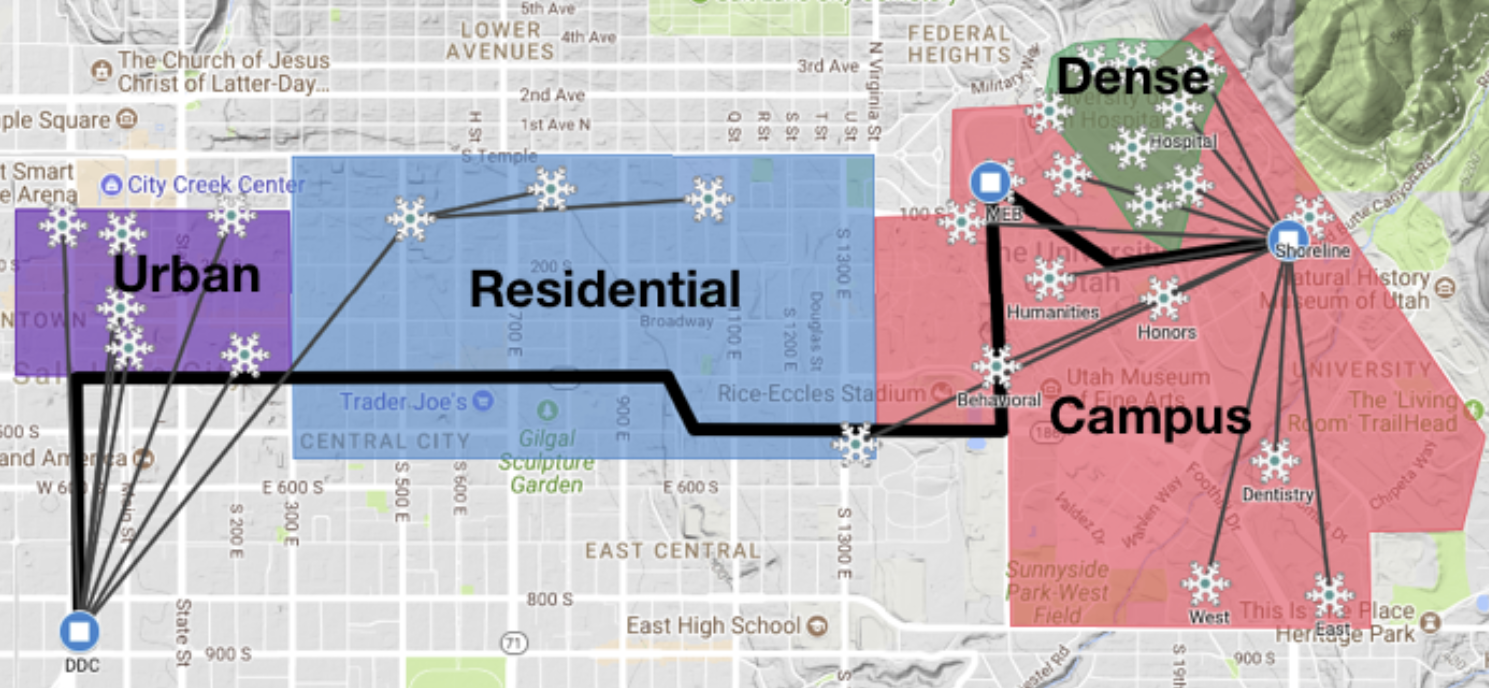
\includegraphics[width=0.9\columnwidth]{powderMap}
  \caption{POWDER city-scale footprint, including a campus, residential, urban, and dense deployments~\cite{Breen+:wintech20}.}
  \label{fig:powdermap}
\end{figure}

\subsection*{Propagation Models}
A propagation model is a tool that is important in the process of planning, developing and analyzing of radio communication networks. 
There is not a one size fits all type of approach when it comes to propagation models. The use of particular propagation models depends
on the parameters available for the chosen area of the propagation study as well as the different parameters of the model. Propagation 
models can be categorized into two common groups: empirical and deterministic models. Deterministic models are based on the physical 
laws of wave propagation to determine the received signal power and often require a detailed map of the propagation environment. Empirical 
models are based on observations and measurements alone and are mainly used to predict path loss.

There is a vast array of propagation models like: Longley-Rice, Okumura-Hata, COST-231, Egli, and others. From the ones listed
Longley-Rice is by far the most widely known and used. In fact, our modeling tool SPLAT! is based on the Longley-Rice 
model~\cite{comparisonof}. The Longley-Rice model is based on electromagnetic theory and on statistical analysis of both terrain features 
and radio measurements. The model can act as an area prediction model or as a point-to-point model. To use the model, one computes the 
additional loss to each path obstruction. These losses are summed and then added to the predicted line of sight path loss which is calculated 
using the Friis transmission equation in SPLAT!~\cite{jeremyclark}.

\subsection*{Unknown Reference}
In the POWDER platform we have uncalibrated radios. This means that when we take power measurements, we will have power 
values with respect to an unknown reference~\cite{pathlossmodels}. The receiver still provides a dB measurement of power, however,
there is no known reference. This proves to be extremely frustrating when comparing data from other places as you simply cannot compare
point-to-point values. A few possible solutions exist to solve this problem. You can calibrate the receiver and transmitter or simply find other
ways of legitimately comparing your data. The latter is used in our results section. 

%%%%%%%%%%%%%%%%%%%%%%%%%%%%%%%%%%%%%%%%%%%%%%%%%%%%%%%%%%%%%%%%%%%%%%%%%%%%%%%

%% End of file.